%%%_* Document preamble
\documentclass[14pt,t,usepdftitle=false,
xcolornames=x11names,svgnames,dvipsnames]{beamer}
\usepackage{fontspec}
\usepackage{listings}
\usepackage{alltt}
%%%_* Simplest theme ever; white background, no widgets
\usetheme{default}
\setbeamertemplate{navigation symbols}{}
\setbeameroption{show notes}
\setbeamertemplate{frametitle}[default][center]
\setbeamersize{text margin left=10mm}
%%%_** Fancy fonts
\setbeamerfont{frametitle}{series=\bfseries}
\setmainfont[Mapping=tex-text]{Warnock Pro}
\setsansfont[Mapping=tex-text,Numbers={OldStyle}]{Cronos Pro}
\setmonofont[Mapping=tex-text]{Inconsolata}
\newcommand{\wackyFont}[1]{
  {\LARGE\fontspec[Mapping=tex-text]{Immi Five O Five Std} #1}}
\newcommand{\subtitleFont}[1]{{\footnotesize #1}}
\newcommand{\slideheading}[1]{
  \begin{center}
    \usebeamerfont{frametitle}
    \usebeamercolor[fg]{frametitle}#1
  \end{center}\vskip-5mm}
\usefonttheme{professionalfonts}
%%%_** Color definitions
\colorlet{comment}{Olive}
\colorlet{string}{SaddleBrown}
\colorlet{keyword}{Navy}
\colorlet{type}{Green}
\colorlet{emph}{Maroon}
\colorlet{input}{Indigo}
\colorlet{error}{DarkRed}
\colorlet{result}{LightSlateGrey}
\colorlet{background}{LightGoldenrodYellow}
\colorlet{hole}{LimeGreen}

%%%_** Listings settings
% "define" Scala
\lstdefinelanguage{scala}{
  morekeywords={abstract,case,catch,class,def,%
    do,else,extends,false,final,finally,%
    for,if,implicit,import,match,mixin,%
    new,null,object,override,package,%
    private,protected,requires,return,sealed,%
    super,this,throw,trait,true,try,%
    type,val,var,while,with,yield},
  otherkeywords={=,=>,<-,<\%,<:,>:,\#,@},
  emph={String,Int,Boolean,Unit,Float,Any,Double,List},
  sensitive=true,
  morecomment=[l]{//},
  morecomment=[n]{/*}{*/},
  morestring=[b]",
  morestring=[b]',
  morestring=[b]"""
}
\lstdefinestyle{scala}{
  language=scala,
  numbers=none,
  numberstyle=\tiny, 
  numbersep=5pt,
  delim=[is][\color{hole}\colorbox{hole}]{(/)}{(/)},
}
\lstdefinestyle{scalarepl}{
  language=scala,
  moredelim=[l][\color{input}]{scala>},
  moredelim=[l][\color{result}]{res},
  frame=single,
  backgroundcolor={\color{background}},
}
\lstdefinestyle{smlrepl}{
  moredelim=[l][\color{input}]{- },
  moredelim=[l][\color{result}]{val },
  moredelim=[l][\color{error}]{uncaught},
  moredelim=[l][\color{error}]{raised},
  moredelim=[s][\color{emph}]{\[}{\]}
}
\lstset{
  columns=flexible,
  showstringspaces=false,
  basicstyle={\small\ttfamily},
  keywordstyle={\bfseries\color{keyword}},
  commentstyle=\color{comment},
  stringstyle=\color{string},
  emphstyle={\color{type}},
  emphstyle={[2]\color{emph}},
  breakatwhitespace=true,
  tabsize=3,
}

%%%_* Metadata
\title{\wackyFont{Futzing with actors (etc.)}}
%\subtitle{\textbf{(and such)}}
\author{Christopher League\\\subtitleFont{Long Island University}}
\date{\subtitleFont{New York Scala Enthusiasts\\A Pattern Language of Concurrency\\27 June 2011}}
%%%_* Document
\begin{document}

\maketitle

\begin{frame}
  \frametitle{Analogous advice}
  \bigskip
  \begin{center}
    
\includegraphics[scale=.56]{tweet-max4f}\\
  \end{center}
\end{frame}


\begin{frame}{Call graph}
  \vspace{-12mm}
  \begin{center}
    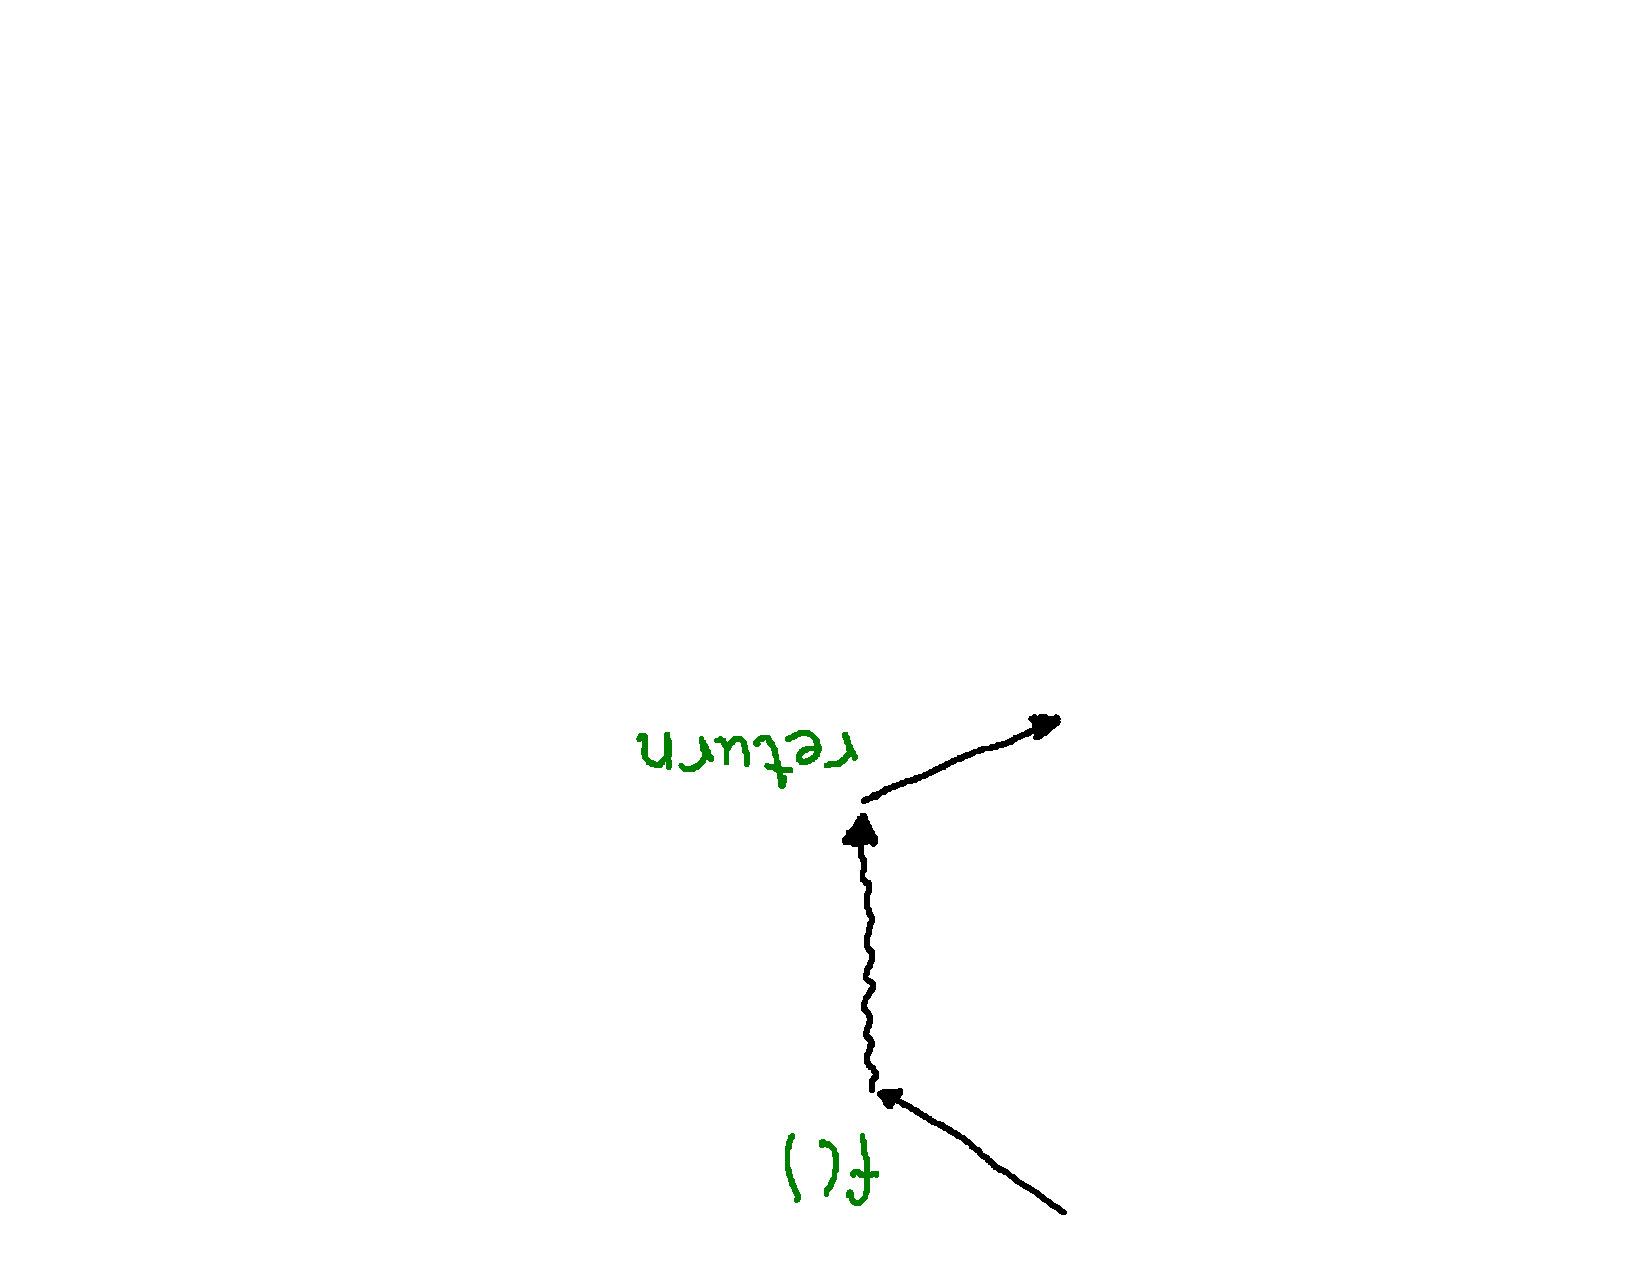
\includegraphics[scale=.4,angle=180]{call-graph.pdf}
  \end{center}
\end{frame}

\begin{frame}{Asynchronicity}
  \vspace{-12mm}
  \begin{center}
    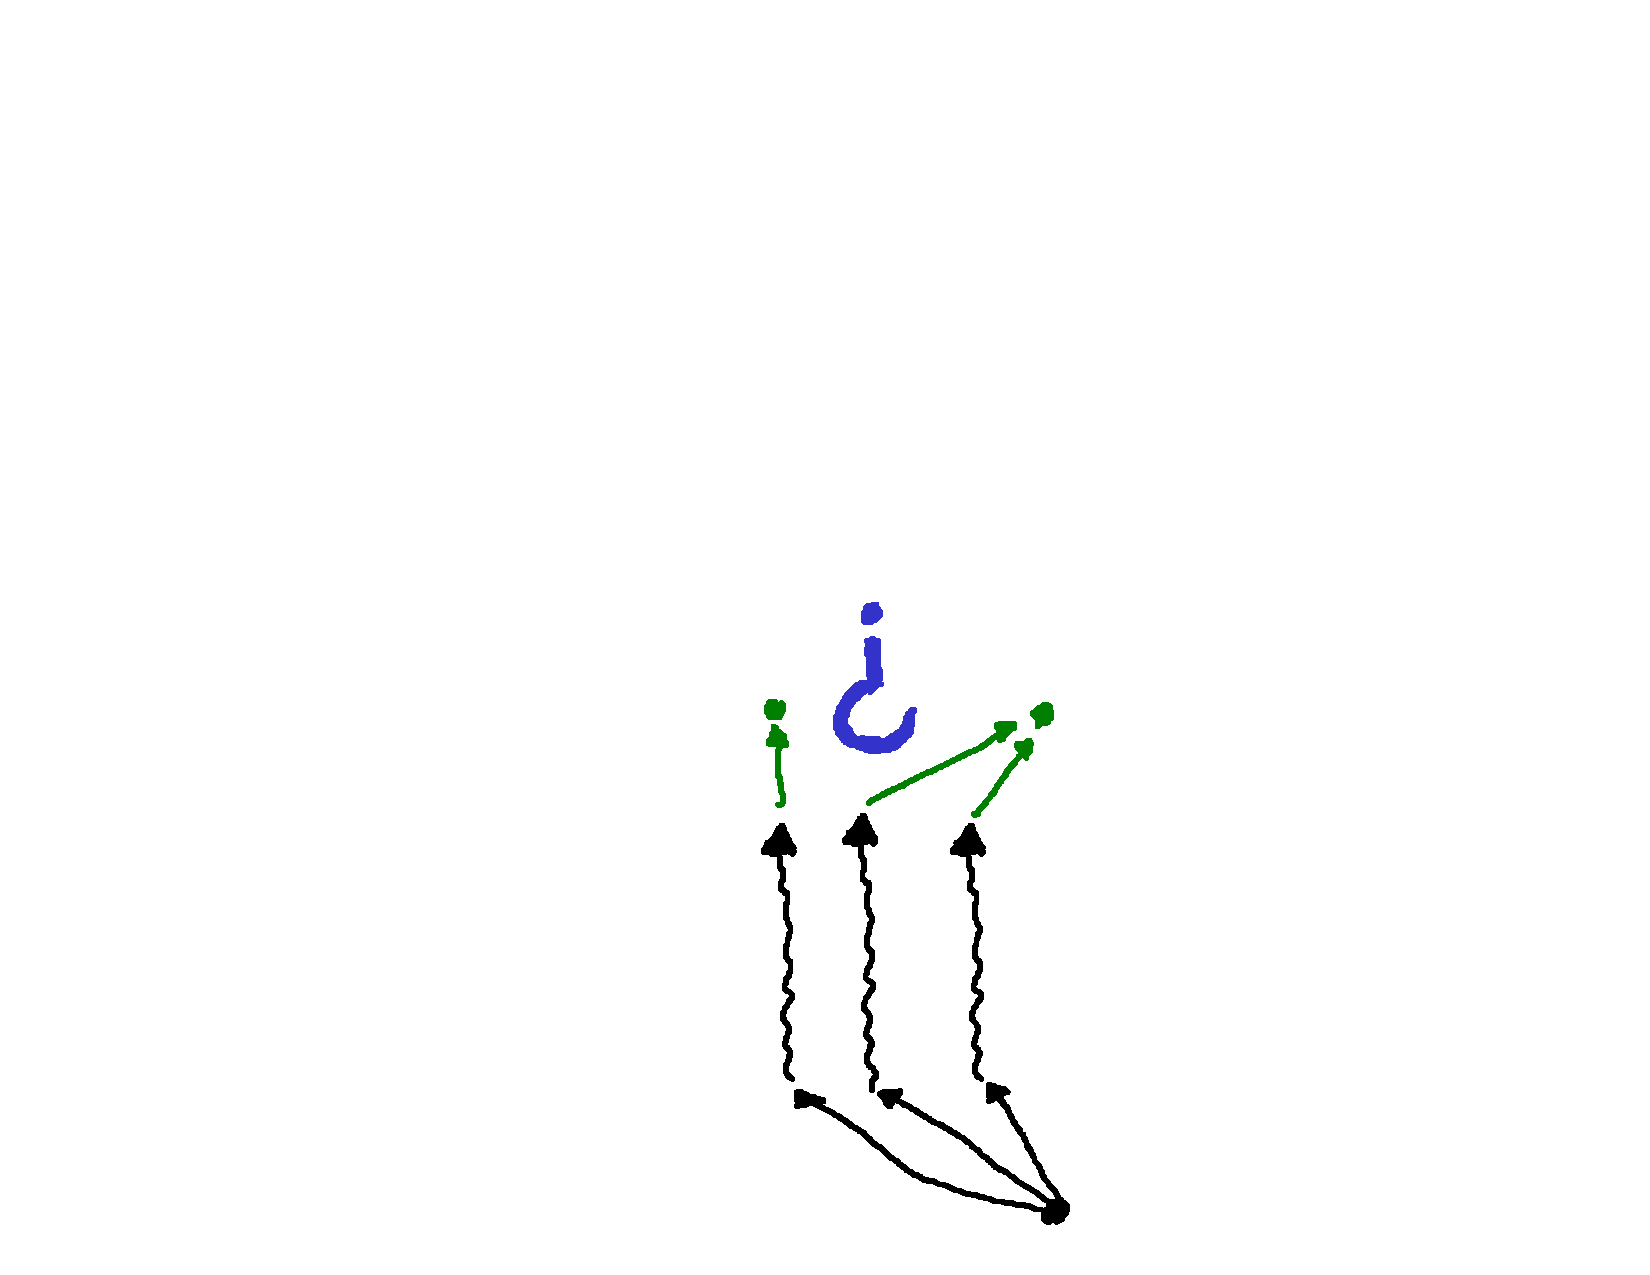
\includegraphics[scale=.4,angle=180]{asynchro.pdf}
  \end{center}
\end{frame}

\begin{frame}[fragile]{Scala actor asynchronicity}
  \begin{lstlisting}[style=scalarepl]
scala> import scala.actors.Actor._

scala> actor{println("TICK")}; println("TOCK")
TOCK
TICK

scala> actor{println("TICK")}; println("TOCK")
TICK
TOCK
  \end{lstlisting}
\end{frame}

\begin{frame}{Scala actors}
  \begin{itemize}
  \item Actors are objects that send/receive messages.
  \item \lstinline:a ! m: \hskip1ex sends message \lstinline!m! to actor
    \lstinline!a!, and returns immediately (fire and forget).
  \item System serializes message receives within actor.
  \item \lstinline:react: does not block thread, but also does not return.
  \item Can arrange computations to follow \lstinline:react: using
    \lstinline:loop:, \lstinline:andThen:.
  \end{itemize}
\end{frame}

\begin{frame}[fragile]{Scala actor messaging}
  \lstinputlisting[style=scala,firstline=2,lastline=15
  ]{../src/main/scala/LoudCounter.scala}
\end{frame}


\begin{frame}[fragile]{Sending replies}
  \lstinputlisting[style=scala,firstline=2,lastline=14
  ]{../src/main/scala/ReplyCounter.scala}
\end{frame}

\begin{frame}[fragile]{Awaiting replies}
  \begin{lstlisting}[style=scalarepl]
scala> counter.getState
res0: scala.actors.Actor.State.Value = Runnable

scala> counter ! Incr
scala> counter.getState
res2: scala.actors.Actor.State.Value = Suspended

scala> counter ! Incr
scala> val f = counter !! Get
f: counter.Future[Any] = <function0>

scala> f()
res5: Any = 2
  \end{lstlisting}
\end{frame}

\begin{frame}[fragile]{Return to sender}
  \begin{lstlisting}[style=scalarepl]
scala> counter ! Incr

scala> val a = actor{
  counter ! Get
  react { case x:Int => println(x) }
}
3
a: scala.actors.Actor = Actor-anon1-@1b17b38

scala> a.getState
res8: scala.actors.Actor.State.Value = Terminated
\end{lstlisting}
\end{frame}

\begin{frame}{Does sender know best?}
  \begin{itemize}
  \item Sometimes awkward for sender to make sense of response.
  \item Instead, allow reply to another arbitrary actor --- 
    we can always specify \lstinline:self:.
  \end{itemize}
\end{frame}

\begin{frame}[fragile]{`Actor-passing style'}
  \lstinputlisting[style=scala,firstline=2,lastline=15
  ]{../src/main/scala/ApsCounter.scala}
\end{frame}

\begin{frame}[fragile]{`Actor-passing style'}
  \begin{lstlisting}[style=scalarepl]
scala> counter ! Incr

scala> counter ! Incr

scala> counter ! Get(actor{
  react{
    case x:Int => println(x)
  }
})

scala>
2
  \end{lstlisting}
  \begin{itemize}
  \item Haven't we seen something like this before?
  \end{itemize}
\end{frame}

\begin{frame}[fragile]{Continuation-passing style}
  \begin{lstlisting}[style=scala]

def factRecur(n: Int): Int =
  if(n > 0) n * factRecur(n-1)
  else 1

def factCPS[A](n: Int, k: Int => A): A =
  if(n > 0) factCPS(n-1, (x:Int) => k(n*x))
  else k(1)
  \end{lstlisting}
  \begin{lstlisting}[style=scalarepl]
scala> factCPS(10, println)
3628800
  \end{lstlisting}
\end{frame}

\begin{frame}[fragile]{Actor-passing factorial}
  \begin{lstlisting}[style=scala]
  def factAPS(n: Int, k: Actor): Unit =
    if(n > 0) factAPS(n-1, actor{
      react{ case x:Int => k ! (x*n) }
    })
    else k ! 1
  \end{lstlisting}
  \begin{lstlisting}[style=scalarepl]
scala> val printer = actor{loop{react{
    case x:Any => println(x)
  }}}
scala> factAPS(7, printer)
5040
scala> factAPS(10, printer)
3628800
  \end{lstlisting}
\end{frame}

\begin{frame}[fragile]{Tree recursion: Fibonacci}
  \begin{lstlisting}[style=scala]
  def fibRecur(n: Int): Int =
    if(n < 2) 1
    else fibRecur(n-1) + fibRecur(n-2)

  def fibCPS[A](n: Int, k: Int => A): A =
    if(n < 2) k(1)
    else fibCPS(n-1, (x:Int) =>
           fibCPS(n-2, (y:Int) =>
             k(x+y)))
  \end{lstlisting}
\end{frame}

\begin{frame}[fragile]{Actor-passing Fibonacci}
  \begin{lstlisting}[style=scala]
  def fibAPS(n: Int, k: Actor): Unit =
    if(n < 2) k ! 1
    else {
      actor{fibAPS(n-1, ???)}
      fibAPS(n-2, ???)
    }
  \end{lstlisting}
  \begin{itemize}
  \item  How to join the results?
  \end{itemize}
\end{frame}

\begin{frame}[fragile]{Actor-passing Fibonacci}
  \begin{lstlisting}[style=scala]
  def fibAPS(n: Int, k: Actor): Unit =
    if(n < 2) k ! 1
    else {
      val join = actor{
        react{case x:Int =>
          react{ case y:Int => k ! (x+y) }}}

      actor{fibAPS(n-1, join)}
      fibAPS(n-2, join)
    }
  \end{lstlisting}
  \begin{itemize}
  \item Pass the {same} actor, that receives both results using
  {nested} react.
  \end{itemize}
\end{frame}

\begin{frame}[fragile]{Ordering results with nested react}
  \begin{itemize}
  \item What if order matters?
  \item \lstinline:react: uses a partial function
    \begin{itemize}
    \item first matching message is used
    \item any other messages remain in mailbox
    \end{itemize}
  \end{itemize}
\end{frame}
\begin{frame}[fragile]{Ordering results with nested react}
  \lstinputlisting[style=scala,firstline=4,lastline=7
  ]{../src/main/scala/OrderedJoin.scala}
  \begin{lstlisting}[style=scalarepl]
scala> orderedJoin ! (1,"Hello")
scala> orderedJoin ! (2,"world")
(Hello,world)

scala> orderedJoin.getState
res3: scala.actors.Actor.State.Value = Terminated
scala> orderedJoin.restart
scala> orderedJoin ! (2,"hacking")
scala> orderedJoin ! (1,"Happy")
(Happy,hacking)
  \end{lstlisting}
\end{frame}

\begin{frame}[fragile]{An expression tree}
  \vspace{-12mm}
  \begin{center}
    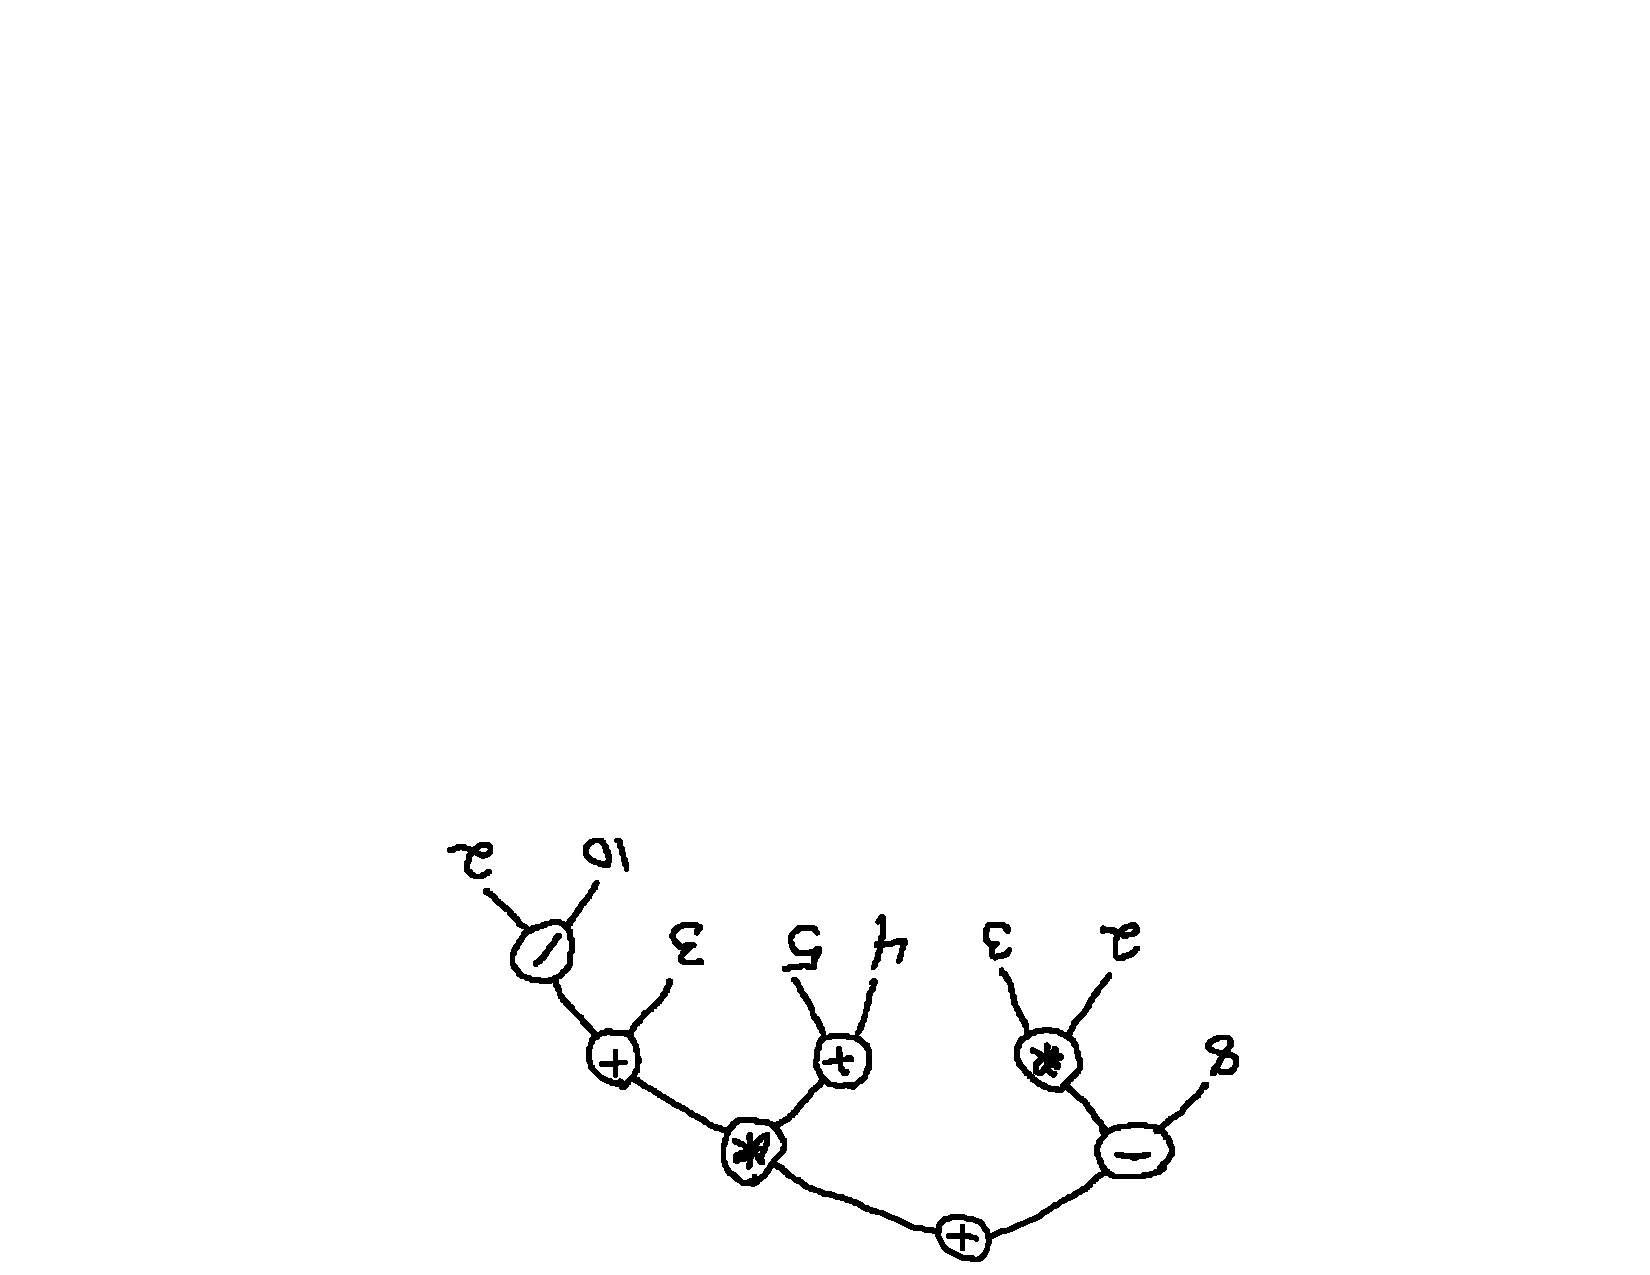
\includegraphics[scale=.5,angle=180]{expr-tree.pdf}
  \end{center}
\end{frame}

\begin{frame}[fragile]{Interpreting operators}
  \lstinputlisting[style=scala,firstline=5,lastline=18
  ]{../src/main/scala/ExprInterp.scala}
\end{frame}

\begin{frame}[fragile]{Building an expression tree}
  \lstinputlisting[style=scala,firstline=19,lastline=32
  ]{../src/main/scala/ExprInterp.scala}
\end{frame}

\begin{frame}[fragile]{Concurrent tree interpretation}
  \lstinputlisting[style=scala,firstline=33,lastline=47
  ]{../src/main/scala/ExprInterp.scala}
\end{frame}

\begin{frame}[fragile]{Concurrent tree interpretation}
  \begin{lstlisting}[style=scalarepl]
scala> interp(eg1, println)
scala>
74
  \end{lstlisting}
  \vspace{-12mm}
  \begin{center}
    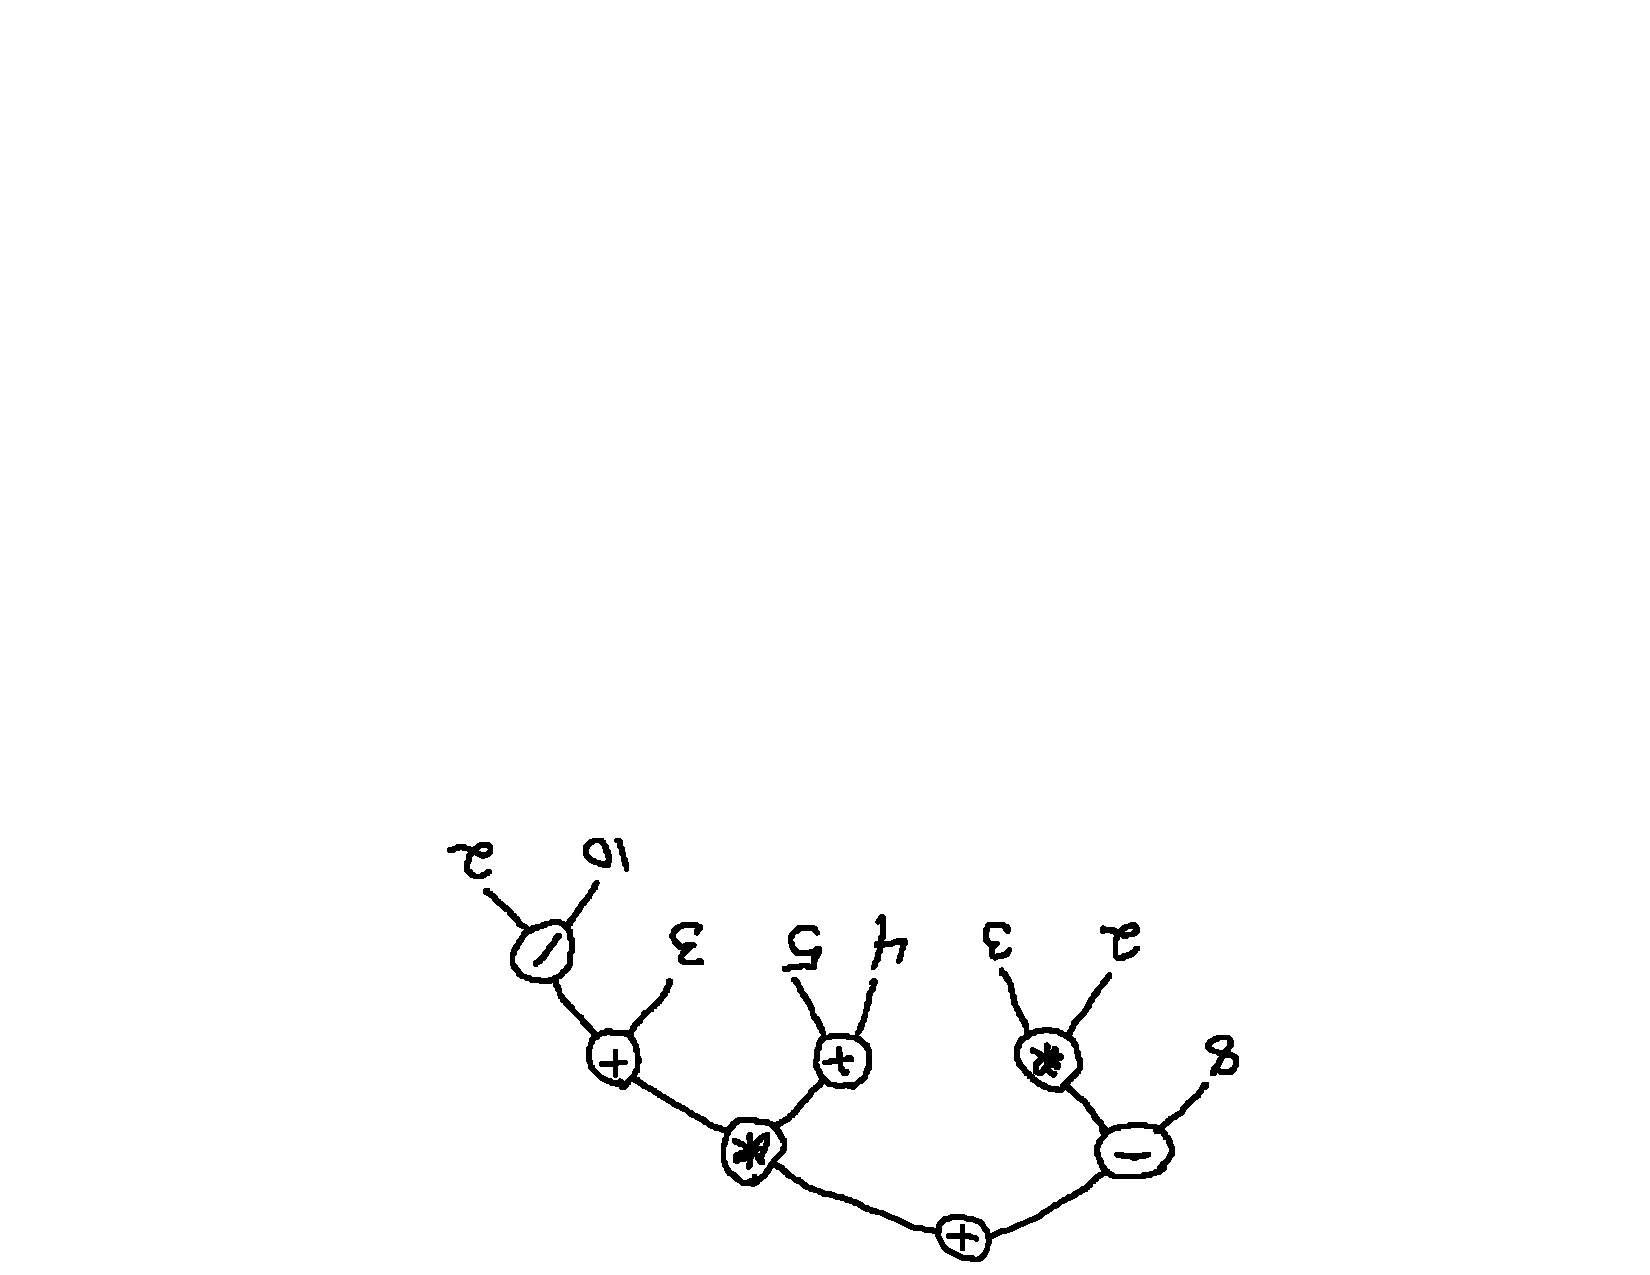
\includegraphics[scale=.5,angle=180]{expr-tree.pdf}
  \end{center}
\end{frame}

\begin{frame}[fragile]{Actors spawned in tree interpreter}
  \vspace{-12mm}
  \begin{center}
    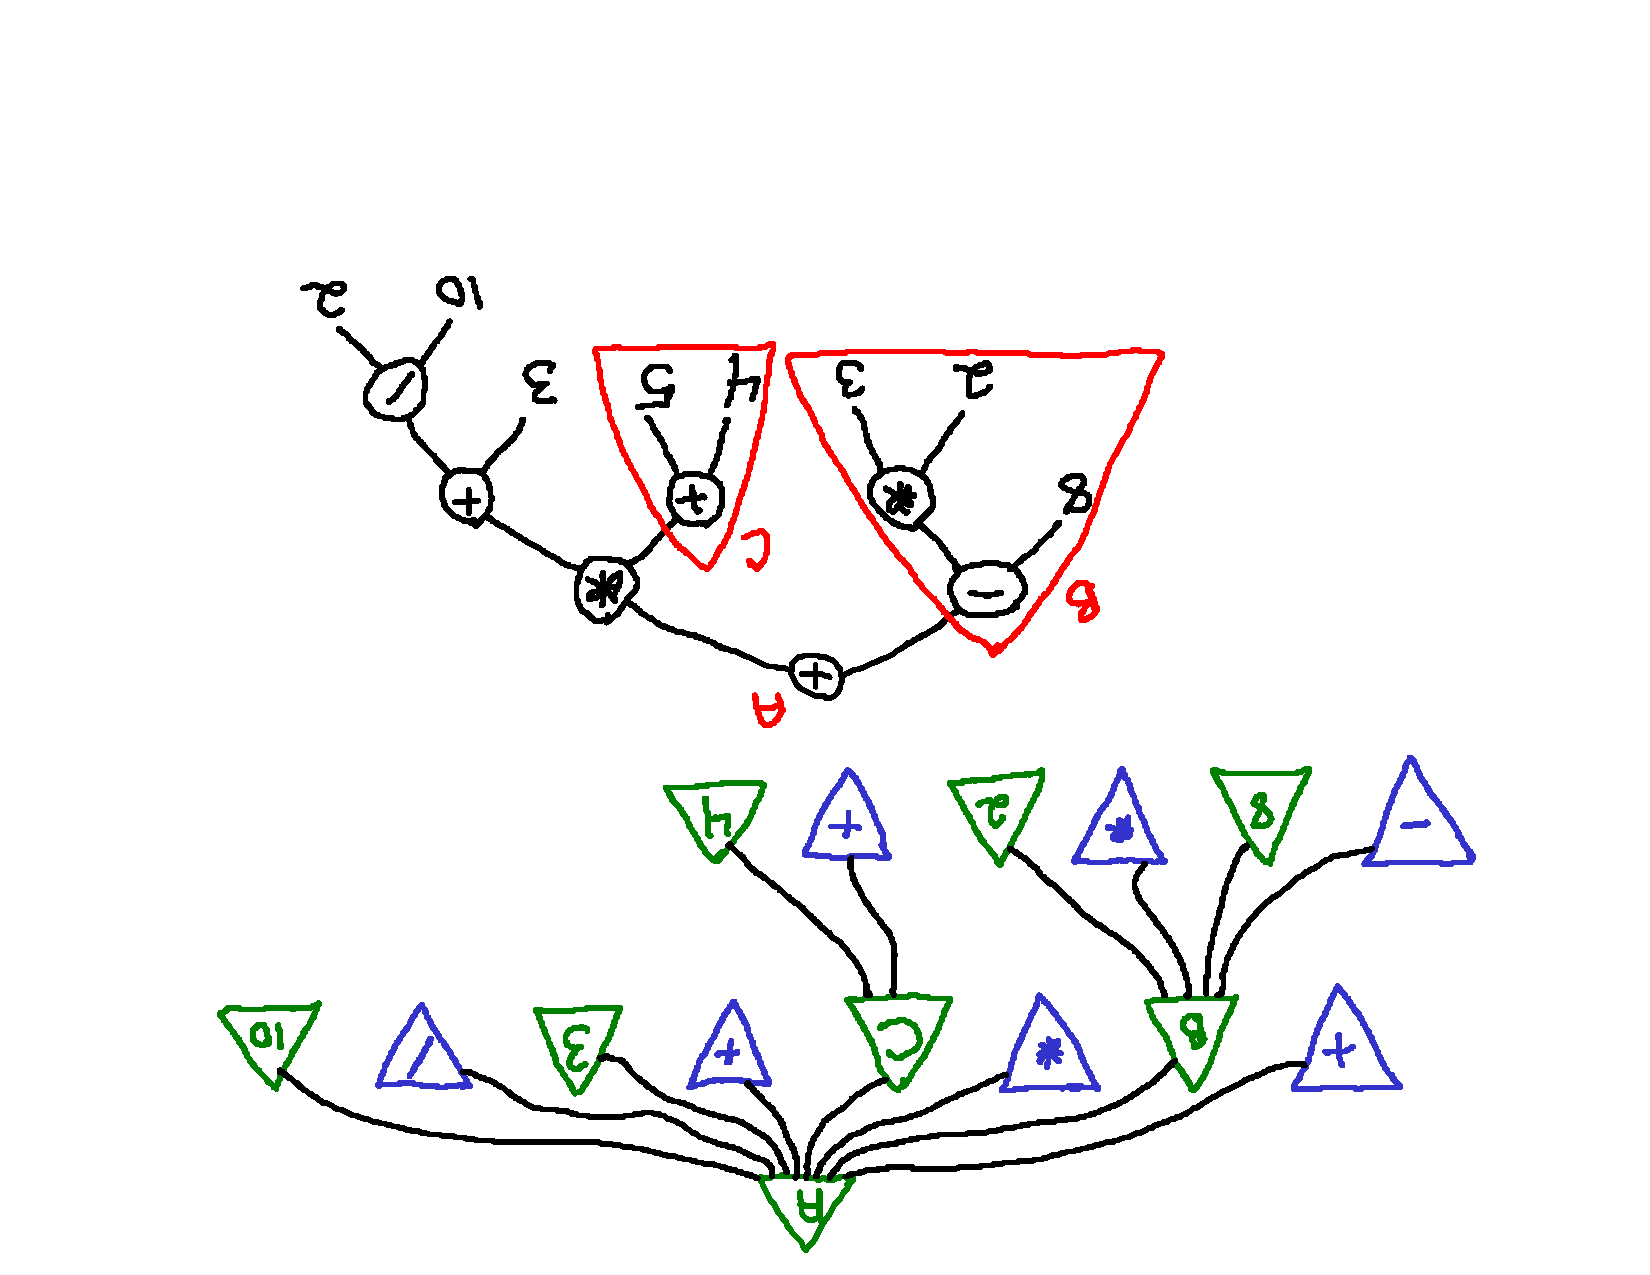
\includegraphics[scale=.4,angle=180]{interp-partition-spawn.pdf}
  \end{center}
\end{frame}

\begin{frame}[fragile]{Messages sent in tree interpreter}
  \vspace{-12mm}
  \begin{center}
    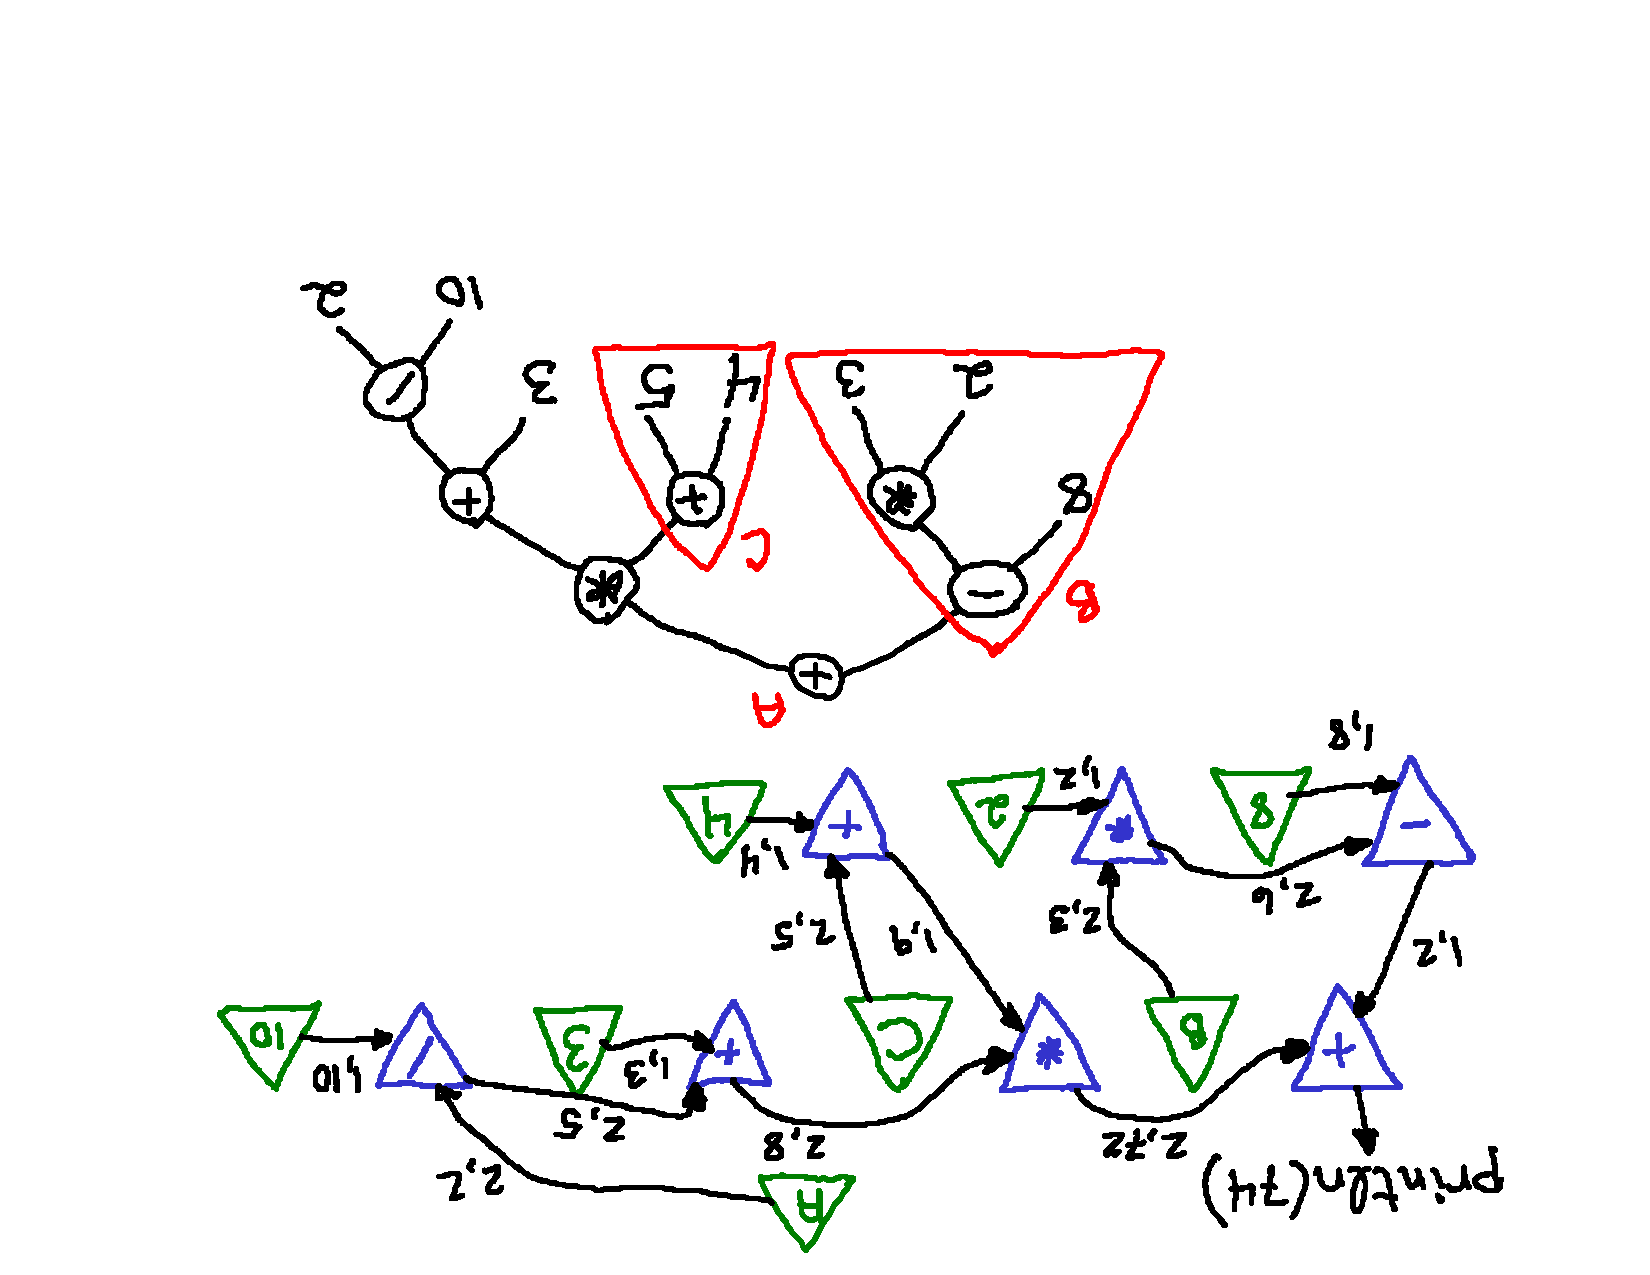
\includegraphics[scale=.4,angle=180]{interp-partition-mesg.pdf}
  \end{center}
\end{frame}

\begin{frame}{Two actors repeatedly rendezvous}
  \begin{itemize}
  \item Next example relies on the flexibility of\\\lstinline:react:,
    \lstinline:andThen:.
  \item Can also be solved with lazy streams or coroutines.
  \end{itemize}
\end{frame}

\begin{frame}[fragile]{Fringe of binary tree}
  \lstinputlisting[style=scala,firstline=7,lastline=17
  ]{../src/main/scala/SameFringe.scala}
\end{frame}

\begin{frame}[fragile]{Fringe of binary tree}
  \lstinputlisting[style=scala,firstline=18,lastline=28
  ]{../src/main/scala/SameFringe.scala}
  \begin{lstlisting}[style=scalarepl]
scala> fringe(t1)
res0: List[Int] = List(1, 2, 3, 4, 5, 6, 7)
scala> fringe(t2)
res1: List[Int] = List(1, 2, 3, 4, 5, 6, 7)
  \end{lstlisting}
\end{frame}

\begin{frame}[fragile]{Do two trees have same fringe?}
  \vspace{-12mm}
  \begin{center}
    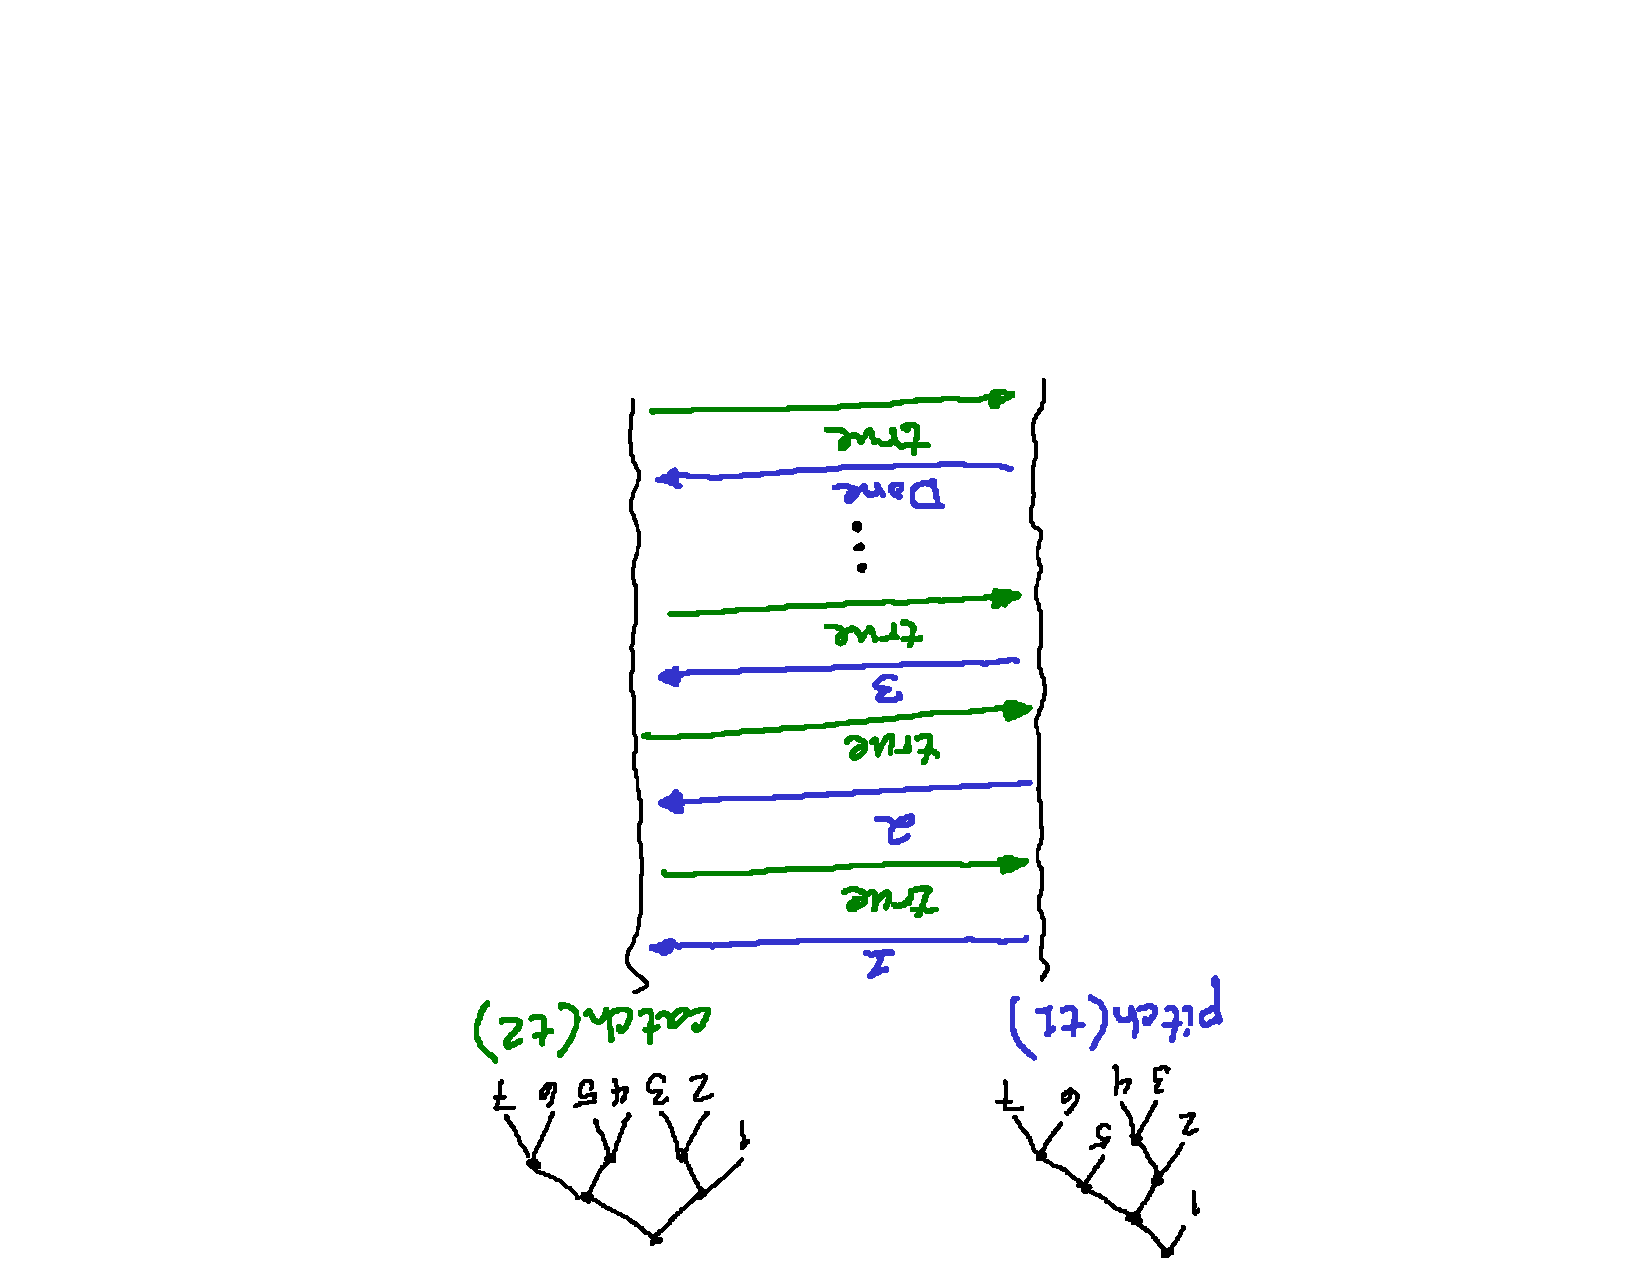
\includegraphics[scale=.45,angle=180]{same-fringe.pdf}
  \end{center}
\end{frame}

\begin{frame}[fragile]{Catcher -- traverse and reply true/false}
  \lstinputlisting[style=scala,firstline=45,lastline=60
  ]{../src/main/scala/SameFringe.scala}
\end{frame}

\begin{frame}[fragile]{Pitcher -- traverse, send, await ack}
  \lstinputlisting[style=scala,firstline=62,lastline=77
  ]{../src/main/scala/SameFringe.scala}
\end{frame}

\begin{frame}[fragile]{Do two trees have same fringe?}
  \begin{lstlisting}[style=scala]
def sameFringe(t1: Tree, t2: Tree, k: Boolean => Unit)
{
  def catch_(t: Tree): Unit = ...
  val catcher = actor { ... }
  def pitch(t: Tree): Unit = ...
  actor { ... }
}
  \end{lstlisting}
  \begin{lstlisting}[style=scalarepl]
scala> sameFringe(t1, t2, println)
scala>
true

scala> sameFringe(t1, t3, println)
false
scala>
  \end{lstlisting}
\end{frame}

\begin{frame}{Lessons}
  \begin{itemize}
  \item Non-blocking actor concurrency\\subverts the call graph, much
    like CPS
  \item Actors are stateful, even without using \lstinline:var:
  \item State may be represented by nested \lstinline:react:
  \item Very cool alternative: \lstinline:scalaz.concurrent.Promise:\\
    Ship computations into the \textbf{future,} using monads!
  \end{itemize}
\end{frame}

\begin{frame}{Thanks!}
  \begin{center}
      \texttt{league@contrapunctus.net}\\
      \texttt{@chrisleague}
  \end{center}
  \begin{itemize}
  \item Code and slides can be made available later;\\ check meetup event page
  \end{itemize}
\end{frame}

\begin{frame}[fragile]{Bonus: A promising interpreter}
  \lstinputlisting[style=scala,firstline=49,lastline=62
  ]{../src/main/scala/ExprInterp.scala}
\end{frame}


%%%%%%%%%%%%%%%%%%%%%%%%%%%%%%%%%%%%%%%%%%%%%%%%%%%%%%%%%%%%
\end{document}
%% Local variables:
%% LaTeX-command: "xelatex"
%% End:
